\section{USUARIOS}
\subsection{Gráfico de dependencias}
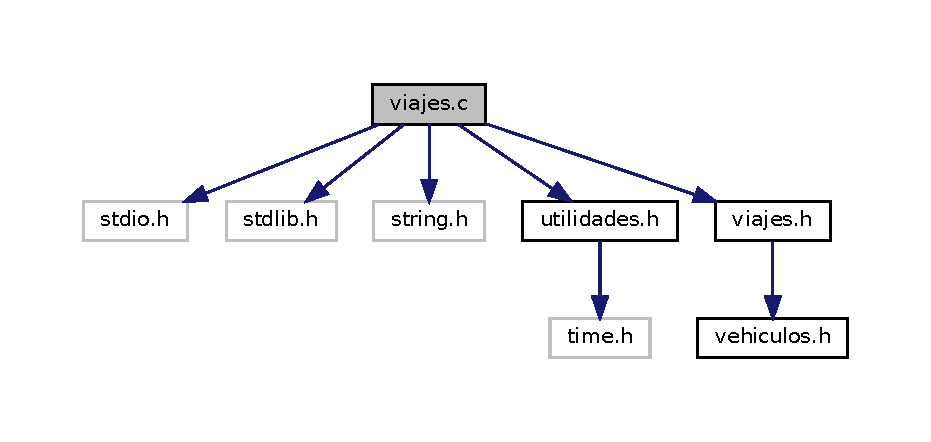
\includegraphics[width=\textwidth, angle=0]{dep/viajes_include.pdf}
\subsection{Estructura de Datos}
\begin{itemize}
    \item \funrf{struct Usuarios}{struct:usuarios}
    \item \funrf{struct vUsuarios}{struct:vusuarios}
\end{itemize}
\subsection{Funciones}
\begin{itemize}
\item \cc{Usuarios* initUsuarios(int * n)}
\item \cc{void saveUsuarios(int n, Usuarios *usuarios)}
\item \cc{void listarUsuarios(vUsuarios* u,vIncidencias* vi)}
\item \cc{void altaUsuario(vUsuarios* v)}
\item \cc{void modificarUsuario(vUsuarios* v,int userId)}
\item \cc{void perfilUsuario(vUsuarios* v,int userId)}
\item \cc{void preguntarIdBaja(vUsuarios* v)}
\item \cc{int printPerfil(vUsuarios* v,int userIndex)}
\item \cc{void reguntarIdModificar(void)}
\end{itemize}
\subsection{Definiciones}
\begin{itemize}
	\item \cc{Usuarios* initUsuarios(int * n)}
	\begin{itemize}
		\item \textbf{Descripcion}
        \begin{itemize}
			\item Inicializa una estructura del tipo Usuarios.
		\end{itemize}
        \item \textbf{Parametros}
		\begin{itemize}
			\item \cc{n} $\rightarrow$ Referencia a la posición del vector que almacena el número de usuarios.
		\end{itemize}
		\item \textbf{Devuelve}
		\begin{itemize}
			\item Un vector con los datos contenidos en el fichero \textbf{Usuarios.txt}.
		\end{itemize}
	\end{itemize}
    \newpage
	\item\cc{void saveUsuarios(int n, Usuarios *usuarios)}
	\begin{itemize}
		\item \textbf{Descripcion}
        \begin{itemize}
			\item Guarda el contenido acutal de una estructura del tipo Usuarios en ficheros.
		\end{itemize}
        \item \textbf{Parametros}
		\begin{itemize}
			\item \cc{n} $\rightarrow$ Referencia a la posición del vector que almacena el número de usuarios.
            \item \cc{usuarios} $\rightarrow$ Puntero a la estructura de usuarios.
		\end{itemize}
	\end{itemize}
    \item\cc{void listarUsuarios(vUsuarios* u,vIncidencias* vi)}
	\begin{itemize}
		\item \textbf{Descripcion}
        \begin{itemize}
			\item Lista el contenido actual de la estructura del tipo Usuarios.
		\end{itemize}
        \item \textbf{Parametros}
		\begin{itemize}
			\item \cc{u} $\rightarrow$ Referencia al vector de Usuarios
            \item \cc{vi} $\rightarrow$ Referencia al vector de Incidencias.
		\end{itemize}
	\end{itemize}
    \item\cc{void altaUsuario(vUsuarios* v)}
	\begin{itemize}
		\item \textbf{Descripcion}
        \begin{itemize}
			\item Añade una nueva línea a la estructura del tipo Usuarios.
		\end{itemize}
        \item \textbf{Parametros}
		\begin{itemize}
			\item \cc{v} $\rightarrow$ Referencia al vector de Usuarios.
		\end{itemize}
	\end{itemize}
	\item\cc{void modificarUsuario(vUsuarios* v,int userId)}
	\begin{itemize}
		\item \textbf{Descripcion}
        \begin{itemize}
			\item Modificar un línea concreta de la estructura del tipo Usuarios.
		\end{itemize}
        \item \textbf{Parametros}
		\begin{itemize}
			\item \cc{v} $\rightarrow$ Referencia al vector de Usuarios.
            \item \cc{userId} $\rightarrow$ Referencia al entero con el indice del usuario seleccionado.
		\end{itemize}
	\end{itemize}
    \item\cc{void perfilUsuario(vUsuarios* v,int userId)}
	\begin{itemize}
		\item \textbf{Descripcion}
        \begin{itemize}
			\item Permite editar al usuario sus datos personales en el sistema y los modifica en la estructura del tipo Usuarios.
		\end{itemize}
        \item \textbf{Parametros}
		\begin{itemize}
			\item \cc{v} $\rightarrow$ Referencia al vector de Usuarios.
            \item \cc{userId} $\rightarrow$ Referencia al entero con el indice del usuario seleccionado.
		\end{itemize}
	\end{itemize}
    \item\cc{void preguntarIdBaja(vUsuarios* v)}
	\begin{itemize}
		\item \textbf{Descripcion}
        \begin{itemize}
			\item Pregunta al administrador qué usuario quiere dar de baja.
		\end{itemize}
        \item \textbf{Parametros}
		\begin{itemize}
			\item \cc{v} $\rightarrow$ Referencia al vector de Usuarios.
		\end{itemize}
	\end{itemize}
    \item\cc{void printPerfil(vUsuarios* v, int userIndex)}
	\begin{itemize}
		\item \textbf{Descripcion}
        \begin{itemize}
			\item Imprime por pantalla el perfil de un usuario en concreto.
		\end{itemize}
        \item \textbf{Parametros}
		\begin{itemize}
			\item \cc{v} $\rightarrow$ Referencia al vector de Usuarios.
            \item \cc{userIndex} $\rightarrow$ Referencia al entero con el indice del usuario seleccionado.
		\end{itemize}
	\end{itemize}
    \item\cc{int preguntarIdModificar(void)}
	\begin{itemize}
		\item \textbf{Descripcion}
        \begin{itemize}
			\item Pregunta al administrador qué usuario desea modificar.
		\end{itemize}
        \item \textbf{Devuelve}
		\begin{itemize}
			\item \cc{tmp} $\rightarrow$ Entero con el id seleccionado.
		\end{itemize}
	\end{itemize}
\end{itemize}
\newpage
